\documentclass{beamer}
\usetheme{metropolis}
\usepackage{graphicx}
\usepackage{subfig}
\usepackage{tcolorbox}
\title{Calculus-Based Physics-2: Electricity, Magnetism, and Thermodynamics (PHYS180-02): Unit 0}
\author{Jordan Hanson}
\institute{Whittier College Department of Physics and Astronomy}

\begin{document}
\maketitle

\begin{frame}{Course Introduction}
\begin{enumerate}
\item Professor Jordan Hanson
\item Contact: jhanson2@whittier.edu, SLC 212
\item Syllabus: Moodle (will examine shortly)
\item Office hours: Tuesdays, 12:00-17:00
\item PHYS150 or PHYS135A and MATH-141B or MATH-142 (concurrent)
\item Text: University Physics Volume 2 (openstax.org)
\end{enumerate}
\end{frame}

\section{Summary}

\begin{frame}{Unit 0 Summary}
\textit{Physics} - $\phi\upsilon\sigma\iota\kappa\acute{\eta}$ - "phusik\'e": \textit{knowledge of nature} \\
from $\phi\acute{\upsilon}\sigma\iota\varsigma$ - "ph\'usis": \textit{nature} \\
\textbf{Reading: Chapters 1 and 2 (for Unit 1)}
\begin{enumerate}
\item Estimation/Approximation
\begin{itemize}
\item \alert{Estimating} the correct order of magnitude
\item \alert{Building} complex quantities
\item \alert{Unit analysis}
\end{itemize}
\item Review of concepts from Newtonian mechanics
\begin{itemize}
\item Kinematics and \alert{Newton's Laws}
\item Work-energy theorem, energy conservation
\item Momentum, conservation of momentum
\end{itemize}
\end{enumerate}
\end{frame}

\begin{frame}{Bonus Essay}
\small
\textbf{\alert{Bonus Essay assignment}}: If you submit a 10-page paper on the history of physics, including references from both online and library sources by the end of the semester, I will replace your lowest midterm score with the grade of the paper.  Example topics:
\begin{itemize}
\item A paper on the Advanced LIGO experiment, and gravitational radiation (Nobel Prize 2017)
\item Development of the idea of energy conservation versus caloric theory by James Joule and others
\item Discovery of the charge to mass ratio of the electron by J.J. Thompson
\item First description of the \textit{photoelectric effect} by Albert Einstein
\end{itemize}
Before beginning the essay, please make an appointment with me in office hours so that we may agree upon a topic.
\end{frame}

\begin{frame}{WAT.}
\centering

\includegraphics[width=0.7\textwidth]{figures/watduck.jpeg}
\end{frame}

\begin{frame}{WAT.}
\centering
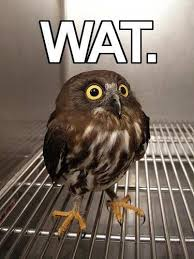
\includegraphics[width=0.4\textwidth]{figures/watowl.jpeg}
\end{frame}

\section{Estimation/Approximation}

\begin{frame}{Estimation/Approximation}
In science and engineering, \alert{estimation} is to obtain a quantity in the absence of precision, informed by rational constraints.
\begin{enumerate}
\item Define relevant \alert{scales}: mg, g, kg
\item Obtain \alert{complex quantities} from simple ones
\begin{itemize}
\item Obtain \textit{areas} and \textit{volumes} from \textit{lengths}
\item Obtain \textit{rates} from \textit{numerators} and \textit{denominators}
\end{itemize}
\item Constrain the unknown with \alert{upper} and \alert{lower} limits
\item Scaling problems: how does a complex quantity depend on other quantities?
\end{enumerate}
\end{frame}

\begin{frame}{Estimation/Approximation}
\small
\begin{columns}[T]
\begin{column}{0.5\textwidth}
\textbf{Choose a reasonable scale}: Estimate the mass of termites in a termite colony.  Assume that the colony is a species known to have $10^6$ individuals (roughly) per colony.
\begin{itemize}
\item A: 0.01 kg
\item B: 0.1 kg
\item C: 1 kg
\item D: 10 kg
\end{itemize}
\end{column}
\begin{column}{0.5\textwidth}
\textbf{Volume/density from other quantities}: An adult humpback whale is about 15 meters long.  What is the mass of a humpback whale? (1 tonne = 1000 kg).
\vspace{0.55cm}
\begin{itemize}
\item A: 200 tonnes
\item B: 30 tonnes
\item C: 3 tonnes
\item D: 1 tonnes
\end{itemize}
\end{column}
\end{columns}
\end{frame}

\begin{frame}{Estimation/Approximation}
\small
\begin{columns}[T]
\begin{column}{0.5\textwidth}
\textbf{Upper and lower bound}: The density of water is 1000 kg/m$^3$.  What is the density of ice, approximately?  (Don't think too hard!)
\begin{itemize}
\item A: 550 kg/m$^3$
\item B: 920 kg/m$^3$
\item C: 1050 kg/m$^3$
\item D: 1200 kg/m$^3$
\end{itemize}
\end{column}
\begin{column}{0.5\textwidth}
\textbf{Volumes from other quantities}: A jar at the coffee shop is filled with coffee beans, and a we can win a prize for guessing the number of beans.  If the radius of the jar is about 4 cm, and the height is about 10 cm, how many beans are in the jar?
\vspace{0.55cm}
\begin{itemize}
\item A: 200
\item B: 2,000
\item C: 10,000
\item D: Um, like, a million...
\end{itemize}
\end{column}
\end{columns}
\end{frame}

\begin{frame}{Estimation/Approximation}
\small
\begin{columns}[T]
\begin{column}{0.5\textwidth}
\textbf{Rates from other quantities}: A student travels from uptown Whittier to SLC in roughly 10 minutes.  What is her average speed?
\begin{itemize}
\item A: 0.1 m/s
\item B: 1 m/s
\item C: 5 m/s
\item D: 10 m/s
\end{itemize}
\end{column}
\begin{column}{0.5\textwidth}
\textbf{Scale}: The distance between the Earth and the sun is 1 AU.  What is the distance between the Sun and Venus?
\vspace{0.55cm}
\begin{itemize}
\item A: 10 million km
\item B: 100 million km
\item C: 0.2 AU
\item D: 0.7 AU
\end{itemize}
\end{column}
\end{columns}
\end{frame}

\begin{frame}{Estimation/Approximation}
\small
\begin{columns}[T]
\begin{column}{0.5\textwidth}
\textbf{Scaling problem}: A balloon has an initial volume of 10 cm$^3$.  It is inflated such that the radius doubles.  What is the new volume?
\begin{itemize}
\item A: 20 cm$^3$
\item B: 40 cm$^3$
\item C: 60 cm$^3$
\item D: 80 cm$^3$
\end{itemize}
\end{column}
\begin{column}{0.5\textwidth}
\textbf{Scaling problem}: If the distance between two massive objects decreases by a factor of 2, by how much does the force of gravity between them change?
\vspace{0.55cm}
\begin{itemize}
\item A: 4
\item B: 8
\item C: 2
\item D: 1
\end{itemize}
\end{column}
\end{columns}
\end{frame}

\begin{frame}{Estimation/Approximation}
\small
\begin{columns}[T]
\begin{column}{0.5\textwidth}
\textbf{Unit analysis}: Which of the following are top speeds of a runner at the end of a sprint?
\begin{itemize}
\item A: 10 m/s$^2$
\item B: 30 kg m/s
\item C: 7 m/s
\item D: 40 miles per hour
\end{itemize}
\textit{What physical quantities do each of the units represent?}
\end{column}
\begin{column}{0.5\textwidth}
\textbf{Unit analysis}: What is $9\times 10^{-3}$ kg m/s in g cm/s?
\vspace{0.55cm}
\begin{itemize}
\item A: 9 g cm/s
\item B: 90 g cm/s
\item C: 900 g cm/s
\item D: 9000 g cm/s
\end{itemize}
\end{column}
\end{columns}
\end{frame}

\section{Vectors}

\begin{frame}{Vectors}
\small
\begin{columns}[T]
\begin{column}{0.5\textwidth}
$\vec{p} = 4\hat{i}+2\hat{j}$.  $\vec{q} = -4\hat{i}+2\hat{j}$.  \\
Compute $\vec{p} + \vec{q}$.
\vspace{0.2cm}
\begin{itemize}
\item A: $4\hat{i}+4\hat{j}$
\item B: $0\hat{i}+4\hat{j}$
\item C: $4\hat{i}+0\hat{j}$
\item D: 0
\end{itemize}
\end{column}
\begin{column}{0.5\textwidth}
$\vec{p} = -1\hat{i}+6\hat{j}$.  $\vec{q} = 3\hat{i}+0.5\hat{j}$.  \\
Compute $\vec{p} \cdot \vec{q}$.
\vspace{0.2cm}
\begin{itemize}
\item A: -1
\item B: 1
\item C: 0
\item D: 3
\end{itemize}
\end{column}
\end{columns}
\end{frame}

\begin{frame}{Vectors}
\textbf{Vector \textit{fields:}} \\
\url{http://user.mendelu.cz/marik/EquationExplorer/vectorfield.html}
\end{frame}

\begin{frame}{Vectors}
\small
\begin{columns}[T]
\begin{column}{0.5\textwidth}
$\vec{f}(x,y) = 4x\hat{i}+2y\hat{j}$.  $\vec{g}(x,y) = 4x\hat{i}-2y\hat{j}$.  \\
Compute $\vec{f} + \vec{g}$.
\vspace{0.2cm}
\begin{itemize}
\item A: $4x\hat{i}+4y\hat{j}$
\item B: $8x\hat{j}$
\item C: $8x\hat{i}$
\item D: $4x\hat{i}$
\end{itemize}
\end{column}
\begin{column}{0.5\textwidth}
$\vec{f}(x,y) = x^2\hat{i}+y^2\hat{j}$.  $\vec{g}(x,y) = -2y\hat{j}$.  \\
Compute $\vec{f} \cdot \vec{g}$.
\vspace{0.2cm}
\begin{itemize}
\item A: $y^3$
\item B: $-2y^2$
\item C: $-2y^3$
\item D: $-2$
\end{itemize}
\end{column}
\end{columns}
\end{frame}

\begin{frame}{Vectors}
What about a dot-product with an \textit{operator}?\\
\begin{equation}
\vec{\nabla} = \left(\frac{\partial}{\partial x},\frac{\partial}{\partial y},\frac{\partial}{\partial z}\right) \label{eq:grad}
\end{equation} \\
Equation \ref{eq:grad} is called the \textit{gradient operator}.  We use it like this:
\begin{align}
\vec{f}(x,y) &= xy \hat{i} - xy \hat{j}\\
\vec{\nabla} \cdot \vec{f} &= y - x
\end{align}
\textit{Notice that the result is a scalar function.}\footnote{We call this operation the divergence of $\vec{f}$.}  It turns out that \textbf{charge} is proportional to the \textbf{divergence} of an electric field.
\end{frame}

\begin{frame}{Vectors}
The \textit{gradient} of a scalar function is \\
\begin{equation}
\nabla f(x,y) = \frac{\partial f}{\partial x}\hat{i}+\frac{\partial f}{\partial y}\hat{j}
\end{equation}
It turns out that the gradient of a scalara function called \textbf{voltage} is proportional to the \textbf{electric field}.  The gradient of \textbf{gravitational potential energy} is proportional to the \textbf{gravitational field.} \\ \vspace{0.5cm}
(Professor: pause here for some examples).
\end{frame}

\begin{frame}{Vectors}
\small
\begin{columns}[T]
\begin{column}{0.5\textwidth}
$f(x,y) = 4x+2y$.  What is $\nabla f(x,y)$?
\begin{itemize}
\item A: $4\hat{i}+2\hat{j}$
\item B: $6$
\item C: $4x\hat{i}+2y\hat{j}$
\item D: $-4\hat{i}-2\hat{j}$
\end{itemize}
\end{column}
\begin{column}{0.5\textwidth}
$\vec{f}(x,y) = -x\hat{i}+y^2\hat{j}$.  What is $\nabla \cdot \vec{f}(x,y)$?
\begin{itemize}
\item A: $-x\hat{i}+y^2\hat{j}$
\item B: $x-y^2$
\item C: $-x+y^2$
\item D: $2y-1$
\end{itemize}
\end{column}
\end{columns}
\end{frame}

\section{Kinematics and Newton's Laws}

\begin{frame}{Kinematics and Newton's Laws}
\small
\textit{Kinematics} - A \alert{description} of the motion of particles and systems \\
\textit{Dynamics} - An \alert{explanation} of the motion of particles and systems \\
\vspace{0.25cm}
What causes an object to move?  \textbf{Forces}.  Forces exist as a result of the \alert{\textbf{interactions}} of objects or systems.\\
\vspace{0.25cm}
\rule{10cm}{0.4pt} \\
\vspace{0.25cm}
\textit{Evolution} - A \alert{description} of the change of biological species \\
\textit{Natural Selection} - An \alert{explanation} of change in biological species \\
\vspace{0.25cm}
What causes species to evolve?  \textbf{Natural selection}.  Natural selection exists because of \alert{election pressures}, \alert{numerous offspring}, and \alert{variation} among offspring.
\end{frame}

\begin{frame}{Kinematics and Newton's Laws}
\textbf{Newton's First Law}: A man slides a palette crate across a concrete floor of his shop.  He exerts a force of 60.0 N, and the box has a constant velocity of 0.5 m/s.  What is the force of friction?
\begin{itemize}
\item A: 60.0 N
\item B: 30.0 N
\item C: -30.0 N
\item D: -60.0 N
\end{itemize}
\end{frame}

\begin{frame}{Kinematics and Newton's Laws}
\textbf{Newton's First Law}: A man walks past a palette crate at rest in his shop.  \textit{From his perspective,} the crate moves at 2 m/s.  What is the net force on the palette crate?
\begin{itemize}
\item A: 30.0 N
\item B: -30.0 N
\item C: 0.0 N
\item D: 60.0 N
\end{itemize}
\end{frame}

\begin{frame}{Kinematics and Newton's Laws}
\textbf{Newton's Second Law}: The crate has a mass of 50 kg, and the force of friction is -10.0 N.  If the pushing force is still 60 N, what is the acceleration?
\begin{itemize}
\item A: 2.0 m/s$^2$
\item B: 1.0 m/s$^2$
\item C: -1.0 m/s$^2$
\item D: -2.0 m/s$^2$
\end{itemize}
\end{frame}

\begin{frame}{Kinematics and Newton's Laws}
\textbf{Kinematics}: If the acceleration is 1.0 m/s$^2$, and the crate begins with a velocity of 1 m/s, what is the velocity after 5 seconds?
\begin{itemize}
\item A: 4 m/s
\item B: 5 m/s
\item C: 6 m/s
\item D: 7 m/s
\end{itemize}
\end{frame}

\begin{frame}{Kinematics and Newton's Laws}
\textbf{Newton's Third Law}: Suppose the crate is now touching a wall, and it is on wheels (so there is no friction).  If a 70 kg man pushes the crate with 100 N, what is the net force on the man by the crate?
\begin{itemize}
\item A: 100 N
\item B: -100 N
\item C: 0 N
\item D: 700 N
\end{itemize}
\end{frame}

\section{Work-Energy Theorem and Conservation of Energy}

\begin{frame}{Definitions of Work}
\begin{tcolorbox}[colback=white,colframe=red!40!blue,title=Physical Definition of Work]
\alert{Let $\vec{F}$ be a force exerted on a system, which is displaced by a displacement $\vec{x}$.  The \textbf{work} done on the system is} \\
\alert{$W = \vec{F} \cdot \vec{x}$} \\
\end{tcolorbox}
The units of work are N m = kg m/s$^2$, or \textit{Joules}. \\
\end{frame}

\begin{frame}{Definitions of Work}
Let $\theta$ be the angle between the force and the displacement.  Then this equation
\begin{equation}
W = \vec{F} \cdot \vec{x}
\end{equation}
becomes
\begin{equation}
W = Fx\cos\theta
\end{equation}
\end{frame}

\begin{frame}{Definitions of Work}
\textbf{Definitions of Work}: Suppose an object is located at $(4,0)$ in a 2D coordinate system.  The object is in a force field $\vec{f} = -4 \hat{i}$.  If the object is moved to the origin by the force, what is the work done?
\begin{itemize}
\item A: 4 J
\item B: -4 J
\item C: 16 J
\item D: -16 J
\end{itemize}
\end{frame}

\begin{frame}{Definitions of Work}
\textbf{Work-Energy theorem}: If the work done is 16 J, what is the final velocity of the object, if the mass is 1.6 kg?
\begin{itemize}
\item A: $\sqrt{20}$ m/s
\item B: $\sqrt{10}$ m/s
\item C: $20$ m/s
\item D: $-10$ m/s
\end{itemize}
\end{frame}

\begin{frame}{Definitions of Work}
What if the force varies over the trajectory of the system?  We simply have to add up each contribution along the trajectory:
\begin{equation}
W = \int_{AB} \vec{F} \cdot d\vec{r}
\end{equation}
\end{frame}

\begin{frame}{Definitions of Work}
\textbf{Definitions of Work}: Suppose an object is located at $(4,0)$ in a 2D coordinate system.  The object is in a force field $\vec{f} = -4x \hat{i}$.  If the object is moved to the origin by the force, what is the work done?
\begin{itemize}
\item A: 16 J
\item B: -16 J
\item C: 32 J
\item D: 4 J
\end{itemize}
(Professor: more examples on the board).
\end{frame}

\begin{frame}{Work and Reversible Processes: the example of friction}
\small
In the first semester we encountered \textit{irreversable} processes: energy lost to \textit{friction}, and energy lost to \textit{drag}. \alert{The irreversable process is a deeper notion in thermal physics}, because it leads to the Second Law of Thermodynamics. \\ \vspace{0.5cm}
\textbf{Group board exercise}: Suppose a system moves at constant speed along a rough surface.  Draw two closed, two-dimensional paths, each describing the trajectory of the system.  A closed path means the system has a final displacement of zero.  Which path requires more work?  \textbf{Key question}: If the speed is constant the entire time, and one path requires more work than the other, what happens to the excess energy (\textit{they have the same final kinetic energy})?
\end{frame}

\begin{frame}{Kinetic Energy and the Work-Energy Theorem}
\textbf{Group board exercise}: A firework of mass 1 kg is launched straight upwards.  The gunpowder releases 500 J of energy.  What is the velocity of the shell as it leaves the launcher?  How high does it fly straight upwards?
\end{frame}

\section{Momentum}

\begin{frame}{Definition of momentum}
Let the momentum of a system be
\begin{equation}
\vec{p} = m \vec{v}
\end{equation}
Newton's second law is then
\begin{equation}
\vec{F}_{Net} = \frac{d\vec{p}}{dt}
\end{equation}
Momentum is a conserved quantity, and in interactions where the kinetic energy is also conserved, we denote them \textit{elastic interactions.} Otherwise, we denote them \textit{inelastic.}  Totally inelastic collisions correspond to maximum kinetic energy lost.
\end{frame}

\begin{frame}{Definition of momentum}
An object that has a small mass and an object that has a large mass have the same momentum. Which mass has the largest kinetic energy?
\begin{itemize}
\item A: The one with the small mass
\item B: The one with the large mass
\item C: If the momentum is the same the kinetic energy is the same
\item D: Cannot determine the answer
\end{itemize}
\textit{Hint:} plug in your own numbers to test your answer.
\end{frame}

\begin{frame}{Momentum}
\textbf{Group board problem:}
Two charged particles, each having opposite sign charge, will always repel each other.  Particle 1 has mass $3m$, and particle 2 has just $m$.  Each approaches the other with speed $v$ (particle 2 is going to the left, particle 1 to the right).  Particle 1 is observed after the collision with speed $-\frac{1}{6}v$.  What is the speed of particle 2?
\end{frame}

\begin{frame}{Thinking about temperature, heat, and thermal physics}
So which parts of Newtonian mechanics are we going to need to understand thermal physics? (Heat, temperature, energy transfer).
\begin{itemize}
\item Newton's laws, momentum and kinetics $\rightarrow$ motions of molecules in gases $\rightarrow$ temperature and heat
\item Work and energy $\rightarrow$ work done by thermal systems $\rightarrow$ energy conservation with heat
\item Irreversable processes $\rightarrow$ energy dissapation $\rightarrow$ entropy
\end{itemize}
\end{frame}

\section{Conclusion}

\begin{frame}{Unit 0 Summary}
\textit{Physics} - $\phi\upsilon\sigma\iota\kappa\acute{\eta}$ - "phusik\'e": \textit{knowledge of nature} \\
from $\phi\acute{\upsilon}\sigma\iota\varsigma$ - "ph\'usis": \textit{nature}
\textbf{Reading: Chapters 1 and 2 (for Unit 1)}
\begin{enumerate}
\item Estimation/Approximation
\begin{itemize}
\item \alert{Estimating} the correct order of magnitude
\item \alert{Building} complex quantities
\item \alert{Unit analysis}
\end{itemize}
\item Review of concepts from Newtonian mechanics
\begin{itemize}
\item Kinematics and \alert{Newton's Laws}
\item Work-energy theorem, energy conservation
\item Momentum, conservation of momentum
\end{itemize}
\end{enumerate}
\end{frame}

\section{Answers}

\begin{frame}{Answers}
\begin{columns}[T]
\begin{column}{0.5\textwidth}
\begin{itemize}
\item 1 kg
\item 30 tonnes
\item 920 kg/m$^3$
\item 2000
\item 1 m/s
\item 0.7 AU
\item 80 cm$^3$
\item 4
\item 900 g cm/s
\item $0\hat{i}+4\hat{j}$
\item 0
\end{itemize}
\end{column}
\begin{column}{0.5\textwidth}
\begin{itemize}
\item $8x\hat{i}$
\item $-2y^3$
\item $4\hat{i}+2\hat{j}$
\item $2y-1$
\item -60.0 N
\item 0.0 N
\item 1.0 m/s$^2$
\item 6 m/s
\item -100 N
\item 16 J
\item $\sqrt{20}$ m/s
\end{itemize}
\end{column}
\end{columns}
\end{frame}

\begin{frame}{Answers, continued}
\begin{columns}[T]
\begin{column}{0.5\textwidth}
\begin{itemize}
\item 32 J
\item The one with the small mass
\end{itemize}
\end{column}
\begin{column}{0.5\textwidth}
\begin{itemize}
\item ...
\end{itemize}
\end{column}
\end{columns}
\end{frame}

\end{document}
